\documentclass[]{article}
\usepackage{lmodern}
\usepackage{amssymb,amsmath}
\usepackage{ifxetex,ifluatex}
\usepackage{fixltx2e} % provides \textsubscript
\ifnum 0\ifxetex 1\fi\ifluatex 1\fi=0 % if pdftex
  \usepackage[T1]{fontenc}
  \usepackage[utf8]{inputenc}
\else % if luatex or xelatex
  \ifxetex
    \usepackage{mathspec}
  \else
    \usepackage{fontspec}
  \fi
  \defaultfontfeatures{Ligatures=TeX,Scale=MatchLowercase}
\fi
% use upquote if available, for straight quotes in verbatim environments
\IfFileExists{upquote.sty}{\usepackage{upquote}}{}
% use microtype if available
\IfFileExists{microtype.sty}{%
\usepackage{microtype}
\UseMicrotypeSet[protrusion]{basicmath} % disable protrusion for tt fonts
}{}
\usepackage[margin=1in]{geometry}
\usepackage{hyperref}
\hypersetup{unicode=true,
            pdftitle={Compulsory exercise 1: Group XYZ},
            pdfauthor={NN1, NN2 and NN3},
            pdfborder={0 0 0},
            breaklinks=true}
\urlstyle{same}  % don't use monospace font for urls
\usepackage{color}
\usepackage{fancyvrb}
\newcommand{\VerbBar}{|}
\newcommand{\VERB}{\Verb[commandchars=\\\{\}]}
\DefineVerbatimEnvironment{Highlighting}{Verbatim}{commandchars=\\\{\}}
% Add ',fontsize=\small' for more characters per line
\usepackage{framed}
\definecolor{shadecolor}{RGB}{248,248,248}
\newenvironment{Shaded}{\begin{snugshade}}{\end{snugshade}}
\newcommand{\KeywordTok}[1]{\textcolor[rgb]{0.13,0.29,0.53}{\textbf{#1}}}
\newcommand{\DataTypeTok}[1]{\textcolor[rgb]{0.13,0.29,0.53}{#1}}
\newcommand{\DecValTok}[1]{\textcolor[rgb]{0.00,0.00,0.81}{#1}}
\newcommand{\BaseNTok}[1]{\textcolor[rgb]{0.00,0.00,0.81}{#1}}
\newcommand{\FloatTok}[1]{\textcolor[rgb]{0.00,0.00,0.81}{#1}}
\newcommand{\ConstantTok}[1]{\textcolor[rgb]{0.00,0.00,0.00}{#1}}
\newcommand{\CharTok}[1]{\textcolor[rgb]{0.31,0.60,0.02}{#1}}
\newcommand{\SpecialCharTok}[1]{\textcolor[rgb]{0.00,0.00,0.00}{#1}}
\newcommand{\StringTok}[1]{\textcolor[rgb]{0.31,0.60,0.02}{#1}}
\newcommand{\VerbatimStringTok}[1]{\textcolor[rgb]{0.31,0.60,0.02}{#1}}
\newcommand{\SpecialStringTok}[1]{\textcolor[rgb]{0.31,0.60,0.02}{#1}}
\newcommand{\ImportTok}[1]{#1}
\newcommand{\CommentTok}[1]{\textcolor[rgb]{0.56,0.35,0.01}{\textit{#1}}}
\newcommand{\DocumentationTok}[1]{\textcolor[rgb]{0.56,0.35,0.01}{\textbf{\textit{#1}}}}
\newcommand{\AnnotationTok}[1]{\textcolor[rgb]{0.56,0.35,0.01}{\textbf{\textit{#1}}}}
\newcommand{\CommentVarTok}[1]{\textcolor[rgb]{0.56,0.35,0.01}{\textbf{\textit{#1}}}}
\newcommand{\OtherTok}[1]{\textcolor[rgb]{0.56,0.35,0.01}{#1}}
\newcommand{\FunctionTok}[1]{\textcolor[rgb]{0.00,0.00,0.00}{#1}}
\newcommand{\VariableTok}[1]{\textcolor[rgb]{0.00,0.00,0.00}{#1}}
\newcommand{\ControlFlowTok}[1]{\textcolor[rgb]{0.13,0.29,0.53}{\textbf{#1}}}
\newcommand{\OperatorTok}[1]{\textcolor[rgb]{0.81,0.36,0.00}{\textbf{#1}}}
\newcommand{\BuiltInTok}[1]{#1}
\newcommand{\ExtensionTok}[1]{#1}
\newcommand{\PreprocessorTok}[1]{\textcolor[rgb]{0.56,0.35,0.01}{\textit{#1}}}
\newcommand{\AttributeTok}[1]{\textcolor[rgb]{0.77,0.63,0.00}{#1}}
\newcommand{\RegionMarkerTok}[1]{#1}
\newcommand{\InformationTok}[1]{\textcolor[rgb]{0.56,0.35,0.01}{\textbf{\textit{#1}}}}
\newcommand{\WarningTok}[1]{\textcolor[rgb]{0.56,0.35,0.01}{\textbf{\textit{#1}}}}
\newcommand{\AlertTok}[1]{\textcolor[rgb]{0.94,0.16,0.16}{#1}}
\newcommand{\ErrorTok}[1]{\textcolor[rgb]{0.64,0.00,0.00}{\textbf{#1}}}
\newcommand{\NormalTok}[1]{#1}
\usepackage{graphicx,grffile}
\makeatletter
\def\maxwidth{\ifdim\Gin@nat@width>\linewidth\linewidth\else\Gin@nat@width\fi}
\def\maxheight{\ifdim\Gin@nat@height>\textheight\textheight\else\Gin@nat@height\fi}
\makeatother
% Scale images if necessary, so that they will not overflow the page
% margins by default, and it is still possible to overwrite the defaults
% using explicit options in \includegraphics[width, height, ...]{}
\setkeys{Gin}{width=\maxwidth,height=\maxheight,keepaspectratio}
\IfFileExists{parskip.sty}{%
\usepackage{parskip}
}{% else
\setlength{\parindent}{0pt}
\setlength{\parskip}{6pt plus 2pt minus 1pt}
}
\setlength{\emergencystretch}{3em}  % prevent overfull lines
\providecommand{\tightlist}{%
  \setlength{\itemsep}{0pt}\setlength{\parskip}{0pt}}
\setcounter{secnumdepth}{0}
% Redefines (sub)paragraphs to behave more like sections
\ifx\paragraph\undefined\else
\let\oldparagraph\paragraph
\renewcommand{\paragraph}[1]{\oldparagraph{#1}\mbox{}}
\fi
\ifx\subparagraph\undefined\else
\let\oldsubparagraph\subparagraph
\renewcommand{\subparagraph}[1]{\oldsubparagraph{#1}\mbox{}}
\fi

%%% Use protect on footnotes to avoid problems with footnotes in titles
\let\rmarkdownfootnote\footnote%
\def\footnote{\protect\rmarkdownfootnote}

%%% Change title format to be more compact
\usepackage{titling}

% Create subtitle command for use in maketitle
\newcommand{\subtitle}[1]{
  \posttitle{
    \begin{center}\large#1\end{center}
    }
}

\setlength{\droptitle}{-2em}

  \title{Compulsory exercise 1: Group XYZ}
    \pretitle{\vspace{\droptitle}\centering\huge}
  \posttitle{\par}
  \subtitle{TMA4268 Statistical Learning V2019}
  \author{NN1, NN2 and NN3}
    \preauthor{\centering\large\emph}
  \postauthor{\par}
      \predate{\centering\large\emph}
  \postdate{\par}
    \date{01 februar, 2019}


\begin{document}
\maketitle

\section{Problem 1: Multiple linear
regression}\label{problem-1-multiple-linear-regression}

\begin{Shaded}
\begin{Highlighting}[]
\KeywordTok{library}\NormalTok{(GLMsData)}
\KeywordTok{data}\NormalTok{(}\StringTok{"lungcap"}\NormalTok{)}
\NormalTok{lungcap}\OperatorTok{$}\NormalTok{Htcm=lungcap}\OperatorTok{$}\NormalTok{Ht}\OperatorTok{*}\FloatTok{2.54}
\NormalTok{modelA =}\StringTok{ }\KeywordTok{lm}\NormalTok{(}\KeywordTok{log}\NormalTok{(FEV) }\OperatorTok{~}\StringTok{ }\NormalTok{Age }\OperatorTok{+}\StringTok{ }\NormalTok{Htcm }\OperatorTok{+}\StringTok{ }\NormalTok{Gender }\OperatorTok{+}\StringTok{ }\NormalTok{Smoke, }\DataTypeTok{data=}\NormalTok{lungcap)}
\KeywordTok{summary}\NormalTok{(modelA)}
\end{Highlighting}
\end{Shaded}

\begin{verbatim}
## 
## Call:
## lm(formula = log(FEV) ~ Age + Htcm + Gender + Smoke, data = lungcap)
## 
## Residuals:
##      Min       1Q   Median       3Q      Max 
## -0.63278 -0.08657  0.01146  0.09540  0.40701 
## 
## Coefficients:
##              Estimate Std. Error t value Pr(>|t|)    
## (Intercept) -1.943998   0.078639 -24.721  < 2e-16 ***
## Age          0.023387   0.003348   6.984  7.1e-12 ***
## Htcm         0.016849   0.000661  25.489  < 2e-16 ***
## GenderM      0.029319   0.011719   2.502   0.0126 *  
## Smoke       -0.046067   0.020910  -2.203   0.0279 *  
## ---
## Signif. codes:  0 '***' 0.001 '**' 0.01 '*' 0.05 '.' 0.1 ' ' 1
## 
## Residual standard error: 0.1455 on 649 degrees of freedom
## Multiple R-squared:  0.8106, Adjusted R-squared:  0.8095 
## F-statistic: 694.6 on 4 and 649 DF,  p-value: < 2.2e-16
\end{verbatim}

\textbf{Q1:}

\textbf{Q2:}

\begin{itemize}
\tightlist
\item
  \texttt{Estimate} - in particular interpretation of \texttt{Intercept}
\item
  \texttt{Std.Error}
\item
  \texttt{Residual\ standard\ error}
\item
  \texttt{F-statistic}
\end{itemize}

\textbf{Q3:}

\textbf{Q4:}

\begin{Shaded}
\begin{Highlighting}[]
\KeywordTok{library}\NormalTok{(ggplot2)}
\CommentTok{# residuls vs fitted}
\KeywordTok{ggplot}\NormalTok{(modelA, }\KeywordTok{aes}\NormalTok{(.fitted, .stdresid)) }\OperatorTok{+}\StringTok{ }\KeywordTok{geom_point}\NormalTok{(}\DataTypeTok{pch =} \DecValTok{21}\NormalTok{) }\OperatorTok{+}
\StringTok{  }\KeywordTok{geom_hline}\NormalTok{(}\DataTypeTok{yintercept =} \DecValTok{0}\NormalTok{, }\DataTypeTok{linetype =} \StringTok{"dashed"}\NormalTok{) }\OperatorTok{+}
\StringTok{  }\KeywordTok{geom_smooth}\NormalTok{(}\DataTypeTok{se =} \OtherTok{FALSE}\NormalTok{, }\DataTypeTok{col =} \StringTok{"red"}\NormalTok{, }\DataTypeTok{size =} \FloatTok{0.5}\NormalTok{, }\DataTypeTok{method =} \StringTok{"loess"}\NormalTok{) }\OperatorTok{+}
\StringTok{  }\KeywordTok{labs}\NormalTok{(}\DataTypeTok{x =} \StringTok{"Fitted values"}\NormalTok{, }\DataTypeTok{y =} \StringTok{"Standardized residuals"}\NormalTok{,}
       \DataTypeTok{title =} \StringTok{"Fitted values vs. Standardized residuals"}\NormalTok{,}
       \DataTypeTok{subtitle =} \KeywordTok{deparse}\NormalTok{(modelA}\OperatorTok{$}\NormalTok{call))}
\end{Highlighting}
\end{Shaded}

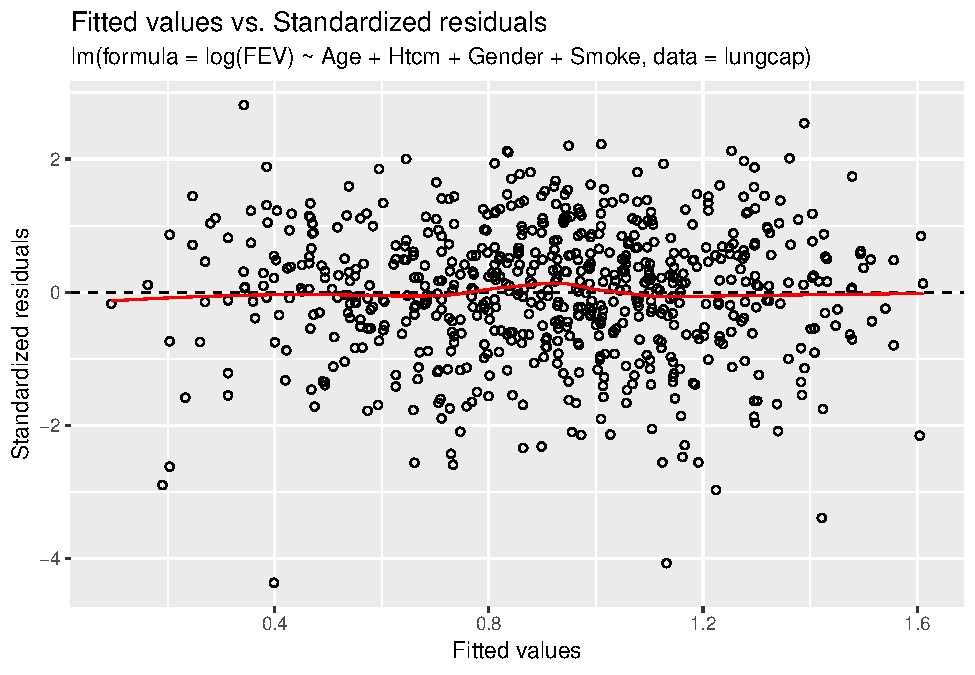
\includegraphics{Compulsory_ex1_files/figure-latex/unnamed-chunk-2-1.pdf}

\begin{Shaded}
\begin{Highlighting}[]
\CommentTok{# qq-plot of residuals}
\KeywordTok{ggplot}\NormalTok{(modelA, }\KeywordTok{aes}\NormalTok{(}\DataTypeTok{sample =}\NormalTok{ .stdresid)) }\OperatorTok{+}
\StringTok{  }\KeywordTok{stat_qq}\NormalTok{(}\DataTypeTok{pch =} \DecValTok{19}\NormalTok{) }\OperatorTok{+}\StringTok{ }
\StringTok{  }\KeywordTok{geom_abline}\NormalTok{(}\DataTypeTok{intercept =} \DecValTok{0}\NormalTok{, }\DataTypeTok{slope =} \DecValTok{1}\NormalTok{, }\DataTypeTok{linetype =} \StringTok{"dotted"}\NormalTok{) }\OperatorTok{+}
\StringTok{  }\KeywordTok{labs}\NormalTok{(}\DataTypeTok{x =} \StringTok{"Theoretical quantiles"}\NormalTok{, }\DataTypeTok{y =} \StringTok{"Standardized residuals"}\NormalTok{, }
       \DataTypeTok{title =} \StringTok{"Normal Q-Q"}\NormalTok{, }\DataTypeTok{subtitle =} \KeywordTok{deparse}\NormalTok{(modelA}\OperatorTok{$}\NormalTok{call))}
\end{Highlighting}
\end{Shaded}

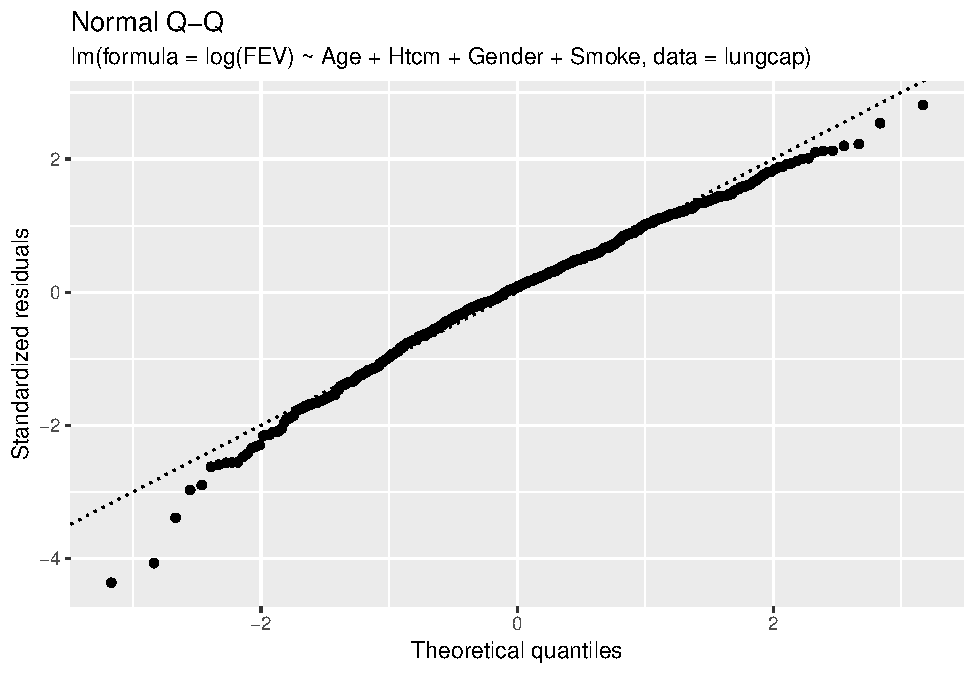
\includegraphics{Compulsory_ex1_files/figure-latex/unnamed-chunk-2-2.pdf}

\begin{Shaded}
\begin{Highlighting}[]
\CommentTok{# normality test}
\KeywordTok{library}\NormalTok{(nortest) }
\KeywordTok{ad.test}\NormalTok{(}\KeywordTok{rstudent}\NormalTok{(modelA))}
\end{Highlighting}
\end{Shaded}

\begin{verbatim}
## 
##  Anderson-Darling normality test
## 
## data:  rstudent(modelA)
## A = 1.9256, p-value = 6.486e-05
\end{verbatim}

\textbf{Q5:}

\begin{Shaded}
\begin{Highlighting}[]
\CommentTok{# here you write your code}
\end{Highlighting}
\end{Shaded}

\textbf{Q6:}

\begin{Shaded}
\begin{Highlighting}[]
\CommentTok{# here you write your code if you have any}
\end{Highlighting}
\end{Shaded}

\textbf{Q7:}

\begin{Shaded}
\begin{Highlighting}[]
\CommentTok{# here you write your code}
\end{Highlighting}
\end{Shaded}

\textbf{Q8:}

\begin{Shaded}
\begin{Highlighting}[]
\NormalTok{new =}\StringTok{ }\KeywordTok{data.frame}\NormalTok{(}\DataTypeTok{Age=}\DecValTok{16}\NormalTok{, }\DataTypeTok{Htcm=}\DecValTok{170}\NormalTok{, }\DataTypeTok{Gender=}\StringTok{"M"}\NormalTok{, }\DataTypeTok{Smoke=}\DecValTok{0}\NormalTok{)}
\end{Highlighting}
\end{Shaded}

\section{Problem 2: Classification}\label{problem-2-classification}

\begin{Shaded}
\begin{Highlighting}[]
\KeywordTok{library}\NormalTok{(class)}\CommentTok{# for function knn}
\KeywordTok{library}\NormalTok{(caret)}\CommentTok{# for confusion matrices}
\end{Highlighting}
\end{Shaded}

\begin{verbatim}
## Loading required package: lattice
\end{verbatim}

\begin{Shaded}
\begin{Highlighting}[]
\NormalTok{raw =}\StringTok{ }\KeywordTok{read.csv}\NormalTok{(}\StringTok{"https://www.math.ntnu.no/emner/TMA4268/2019v/data/tennis.csv"}\NormalTok{)}
\NormalTok{M =}\StringTok{ }\KeywordTok{na.omit}\NormalTok{(}\KeywordTok{data.frame}\NormalTok{(}\DataTypeTok{y=}\KeywordTok{as.factor}\NormalTok{(raw}\OperatorTok{$}\NormalTok{Result),}
                       \DataTypeTok{x1=}\NormalTok{raw}\OperatorTok{$}\NormalTok{ACE.}\DecValTok{1}\OperatorTok{-}\NormalTok{raw}\OperatorTok{$}\NormalTok{UFE.}\DecValTok{1}\OperatorTok{-}\NormalTok{raw}\OperatorTok{$}\NormalTok{DBF.}\DecValTok{1}\NormalTok{, }
                       \DataTypeTok{x2=}\NormalTok{raw}\OperatorTok{$}\NormalTok{ACE.}\DecValTok{2}\OperatorTok{-}\NormalTok{raw}\OperatorTok{$}\NormalTok{UFE.}\DecValTok{2}\OperatorTok{-}\NormalTok{raw}\OperatorTok{$}\NormalTok{DBF.}\DecValTok{2}\NormalTok{))}
\KeywordTok{set.seed}\NormalTok{(}\DecValTok{4268}\NormalTok{) }\CommentTok{# for reproducibility}
\NormalTok{tr =}\StringTok{ }\KeywordTok{sample.int}\NormalTok{(}\KeywordTok{nrow}\NormalTok{(M),}\KeywordTok{nrow}\NormalTok{(M)}\OperatorTok{/}\DecValTok{2}\NormalTok{)}
\NormalTok{trte=}\KeywordTok{rep}\NormalTok{(}\DecValTok{1}\NormalTok{,}\KeywordTok{nrow}\NormalTok{(M))}
\NormalTok{trte[tr]=}\DecValTok{0}
\NormalTok{Mdf=}\KeywordTok{data.frame}\NormalTok{(M,}\StringTok{"istest"}\NormalTok{=}\KeywordTok{as.factor}\NormalTok{(trte))}
\end{Highlighting}
\end{Shaded}

\textbf{Q9:}

\textbf{Q10:}

\begin{Shaded}
\begin{Highlighting}[]
\CommentTok{# here you write your code}
\end{Highlighting}
\end{Shaded}

\begin{Shaded}
\begin{Highlighting}[]
\KeywordTok{set.seed}\NormalTok{(}\DecValTok{0}\NormalTok{)}
\NormalTok{ks =}\StringTok{ }\DecValTok{1}\OperatorTok{:}\DecValTok{30} \CommentTok{# Choose K from 1 to 30.}
\NormalTok{idx =}\StringTok{ }\KeywordTok{createFolds}\NormalTok{(M[tr,}\DecValTok{1}\NormalTok{], }\DataTypeTok{k=}\DecValTok{5}\NormalTok{) }\CommentTok{# Divide the training data into 5 folds.}
\CommentTok{# "Sapply" is a more efficient for-loop. }
\CommentTok{# We loop over each fold and each value in "ks"}
\CommentTok{# and compute error rates for each combination.}
\CommentTok{# All the error rates are stored in the matrix "cv", }
\CommentTok{# where folds are rows and values of $K$ are columns.}
\NormalTok{cv =}\StringTok{ }\KeywordTok{sapply}\NormalTok{(ks, }\ControlFlowTok{function}\NormalTok{(k)\{ }
  \KeywordTok{sapply}\NormalTok{(}\KeywordTok{seq_along}\NormalTok{(idx), }\ControlFlowTok{function}\NormalTok{(j) \{}
\NormalTok{    yhat =}\StringTok{ }\NormalTok{class}\OperatorTok{::}\KeywordTok{knn}\NormalTok{(}\DataTypeTok{train=}\NormalTok{M[tr[ }\OperatorTok{-}\NormalTok{idx[[j]] ], }\OperatorTok{-}\DecValTok{1}\NormalTok{],}
               \DataTypeTok{cl=}\NormalTok{M[tr[ }\OperatorTok{-}\NormalTok{idx[[j]] ], }\DecValTok{1}\NormalTok{],}
               \DataTypeTok{test=}\NormalTok{M[tr[ idx[[j]] ], }\OperatorTok{-}\DecValTok{1}\NormalTok{], }\DataTypeTok{k =}\NormalTok{ k)}
    \KeywordTok{mean}\NormalTok{(M[tr[ idx[[j]] ], }\DecValTok{1}\NormalTok{] }\OperatorTok{!=}\StringTok{ }\NormalTok{yhat)}
\NormalTok{  \})}
\NormalTok{\})}
\end{Highlighting}
\end{Shaded}

\textbf{Q11:}

\begin{Shaded}
\begin{Highlighting}[]
\NormalTok{cv.e =}\StringTok{ }\CommentTok{# fill in}
\NormalTok{cv.se =}\StringTok{ }\CommentTok{#fill in}
\NormalTok{k.min =}\StringTok{ }\CommentTok{# fill in}
\end{Highlighting}
\end{Shaded}

\textbf{Q12:}

\begin{Shaded}
\begin{Highlighting}[]
\KeywordTok{library}\NormalTok{(colorspace)}
\NormalTok{co =}\StringTok{ }\KeywordTok{rainbow_hcl}\NormalTok{(}\DecValTok{3}\NormalTok{)}
\KeywordTok{par}\NormalTok{(}\DataTypeTok{mar=}\KeywordTok{c}\NormalTok{(}\DecValTok{4}\NormalTok{,}\DecValTok{4}\NormalTok{,}\DecValTok{1}\NormalTok{,}\DecValTok{1}\NormalTok{)}\OperatorTok{+}\NormalTok{.}\DecValTok{1}\NormalTok{, }\DataTypeTok{mgp =} \KeywordTok{c}\NormalTok{(}\DecValTok{3}\NormalTok{, }\DecValTok{1}\NormalTok{, }\DecValTok{0}\NormalTok{))}
\KeywordTok{plot}\NormalTok{(ks, cv.e, }\DataTypeTok{type=}\StringTok{"o"}\NormalTok{, }\DataTypeTok{pch =} \DecValTok{16}\NormalTok{, }\DataTypeTok{ylim =} \KeywordTok{c}\NormalTok{(}\DecValTok{0}\NormalTok{, }\FloatTok{0.7}\NormalTok{), }\DataTypeTok{col =}\NormalTok{ co[}\DecValTok{2}\NormalTok{],}
     \DataTypeTok{xlab =} \StringTok{"Number of neighbors"}\NormalTok{, }\DataTypeTok{ylab=}\StringTok{"Misclassification error"}\NormalTok{)}
\KeywordTok{arrows}\NormalTok{(ks, cv.e}\OperatorTok{-}\NormalTok{cv.se, ks, cv.e}\OperatorTok{+}\NormalTok{cv.se, }\DataTypeTok{angle=}\DecValTok{90}\NormalTok{, }\DataTypeTok{length=}\NormalTok{.}\DecValTok{03}\NormalTok{, }\DataTypeTok{code=}\DecValTok{3}\NormalTok{, }\DataTypeTok{col=}\NormalTok{co[}\DecValTok{2}\NormalTok{])}
\KeywordTok{lines}\NormalTok{(ks, train.e, }\DataTypeTok{type=}\StringTok{"o"}\NormalTok{, }\DataTypeTok{pch =} \DecValTok{16}\NormalTok{, }\DataTypeTok{ylim =} \KeywordTok{c}\NormalTok{(}\FloatTok{0.5}\NormalTok{, }\FloatTok{0.7}\NormalTok{), }\DataTypeTok{col =}\NormalTok{ co[}\DecValTok{3}\NormalTok{])}
\KeywordTok{lines}\NormalTok{(ks, test.e, }\DataTypeTok{type=}\StringTok{"o"}\NormalTok{, }\DataTypeTok{pch =} \DecValTok{16}\NormalTok{, }\DataTypeTok{ylim =} \KeywordTok{c}\NormalTok{(}\FloatTok{0.5}\NormalTok{, }\FloatTok{0.7}\NormalTok{), }\DataTypeTok{col =}\NormalTok{ co[}\DecValTok{1}\NormalTok{])}
\KeywordTok{legend}\NormalTok{(}\StringTok{"topright"}\NormalTok{, }\DataTypeTok{legend =} \KeywordTok{c}\NormalTok{(}\StringTok{"Test"}\NormalTok{, }\StringTok{"5-fold CV"}\NormalTok{, }\StringTok{"Training"}\NormalTok{), }\DataTypeTok{lty =} \DecValTok{1}\NormalTok{, }\DataTypeTok{col=}\NormalTok{co)}
\end{Highlighting}
\end{Shaded}

\textbf{Q13:}

\begin{Shaded}
\begin{Highlighting}[]
\NormalTok{k =}\StringTok{ }\KeywordTok{tail}\NormalTok{(}\KeywordTok{which}\NormalTok{(cv.e }\OperatorTok{<}\StringTok{ }\NormalTok{cv.e[k.min] }\OperatorTok{+}\StringTok{ }\NormalTok{cv.se[k.min]), }\DecValTok{1}\NormalTok{)}
\NormalTok{size =}\StringTok{ }\DecValTok{100}
\NormalTok{xnew =}\StringTok{ }\KeywordTok{apply}\NormalTok{(M[tr,}\OperatorTok{-}\DecValTok{1}\NormalTok{], }\DecValTok{2}\NormalTok{, }\ControlFlowTok{function}\NormalTok{(X) }\KeywordTok{seq}\NormalTok{(}\KeywordTok{min}\NormalTok{(X), }\KeywordTok{max}\NormalTok{(X), }\DataTypeTok{length.out=}\NormalTok{size))}
\NormalTok{grid =}\StringTok{ }\KeywordTok{expand.grid}\NormalTok{(xnew[,}\DecValTok{1}\NormalTok{], xnew[,}\DecValTok{2}\NormalTok{])}
\NormalTok{grid.yhat =}\StringTok{ }\KeywordTok{knn}\NormalTok{(M[tr,}\OperatorTok{-}\DecValTok{1}\NormalTok{], M[tr,}\DecValTok{1}\NormalTok{], }\DataTypeTok{k=}\NormalTok{k, }\DataTypeTok{test=}\NormalTok{grid)}
\NormalTok{np =}\StringTok{ }\DecValTok{300}
\KeywordTok{par}\NormalTok{(}\DataTypeTok{mar=}\KeywordTok{rep}\NormalTok{(}\DecValTok{2}\NormalTok{,}\DecValTok{4}\NormalTok{), }\DataTypeTok{mgp =} \KeywordTok{c}\NormalTok{(}\DecValTok{1}\NormalTok{, }\DecValTok{1}\NormalTok{, }\DecValTok{0}\NormalTok{))}
\KeywordTok{contour}\NormalTok{(xnew[,}\DecValTok{1}\NormalTok{], xnew[,}\DecValTok{2}\NormalTok{], }\DataTypeTok{z =} \KeywordTok{matrix}\NormalTok{(grid.yhat, size), }\DataTypeTok{levels=}\NormalTok{.}\DecValTok{5}\NormalTok{, }
        \DataTypeTok{xlab=}\KeywordTok{expression}\NormalTok{(}\StringTok{"x"}\NormalTok{[}\DecValTok{1}\NormalTok{]), }\DataTypeTok{ylab=}\KeywordTok{expression}\NormalTok{(}\StringTok{"x"}\NormalTok{[}\DecValTok{2}\NormalTok{]), }\DataTypeTok{axes=}\OtherTok{FALSE}\NormalTok{,}
        \DataTypeTok{main =} \KeywordTok{paste0}\NormalTok{(k,}\StringTok{"-nearest neighbors"}\NormalTok{), }\DataTypeTok{cex=}\FloatTok{1.2}\NormalTok{, }\DataTypeTok{labels=}\StringTok{""}\NormalTok{)}
\KeywordTok{points}\NormalTok{(grid, }\DataTypeTok{pch=}\StringTok{"."}\NormalTok{, }\DataTypeTok{cex=}\DecValTok{1}\NormalTok{, }\DataTypeTok{col=}\NormalTok{grid.yhat)}
\KeywordTok{points}\NormalTok{(M[}\DecValTok{1}\OperatorTok{:}\NormalTok{np,}\OperatorTok{-}\DecValTok{1}\NormalTok{], }\DataTypeTok{col=}\KeywordTok{factor}\NormalTok{(M[}\DecValTok{1}\OperatorTok{:}\NormalTok{np,}\DecValTok{1}\NormalTok{]), }\DataTypeTok{pch =} \DecValTok{1}\NormalTok{, }\DataTypeTok{lwd =} \FloatTok{1.5}\NormalTok{)}
\KeywordTok{legend}\NormalTok{(}\StringTok{"topleft"}\NormalTok{, }\KeywordTok{c}\NormalTok{(}\StringTok{"Player 1 wins"}\NormalTok{, }\StringTok{"Player 2 wins"}\NormalTok{), }
       \DataTypeTok{col=}\KeywordTok{c}\NormalTok{(}\StringTok{"red"}\NormalTok{, }\StringTok{"black"}\NormalTok{), }\DataTypeTok{pch=}\DecValTok{1}\NormalTok{)}
\KeywordTok{box}\NormalTok{()}
\end{Highlighting}
\end{Shaded}

\textbf{Q14:}

\begin{Shaded}
\begin{Highlighting}[]
\NormalTok{K=}\CommentTok{# your choice from Q13}
\StringTok{  }
\CommentTok{# knn with prob=TRUE outputs the probability of the winning class}
\CommentTok{# therefore we have to do an extra step to get the probability of player 1 winning}
\NormalTok{KNNclass=class}\OperatorTok{::}\KeywordTok{knn}\NormalTok{(}\DataTypeTok{train=}\NormalTok{M[tr,}\OperatorTok{-}\DecValTok{1}\NormalTok{], }\DataTypeTok{cl=}\NormalTok{M[tr,}\DecValTok{1}\NormalTok{], }\DataTypeTok{test=}\NormalTok{M[}\OperatorTok{-}\NormalTok{tr,}\OperatorTok{-}\DecValTok{1}\NormalTok{], }\DataTypeTok{k =}\NormalTok{ K,}\DataTypeTok{prob=}\OtherTok{TRUE}\NormalTok{)}
\NormalTok{KNNprobwinning=}\KeywordTok{attributes}\NormalTok{(KNNclass)}\OperatorTok{$}\NormalTok{prob}
\NormalTok{KNNprob=}\StringTok{ }\KeywordTok{ifelse}\NormalTok{(KNNclass }\OperatorTok{==}\StringTok{ "0"}\NormalTok{, }\DecValTok{1}\OperatorTok{-}\NormalTok{KNNprobwinning, KNNprobwinning)}
\CommentTok{# now KNNprob has probability that player 1 wins, for all matches in the test set}

\KeywordTok{library}\NormalTok{(pROC)}
\CommentTok{# now you use predictor=KNNprob and response=M[-tr,1] }
\CommentTok{# in your call to the function roc in the pROC library}
\end{Highlighting}
\end{Shaded}

\textbf{Q15:}

\begin{Shaded}
\begin{Highlighting}[]
\CommentTok{# here you write your code}
\end{Highlighting}
\end{Shaded}

\section{Problem 3: Bias-variance
trade-off}\label{problem-3-bias-variance-trade-off}

Here you see how to write formulas with latex (needed below) \[
\hat{\boldsymbol \beta}=({\bf X}^T{\bf X})^{-1}{\bf X}^T{\bf Y}
\]

\textbf{Q16:}

\textbf{Q17:}

\textbf{Q18:}
\[\text{E}[(Y_0-\hat{f}({\bf x}_0))^2]=[\text{E}(\hat{f}({\bf x}_0)-f({\bf x}_0)]^2+\text{Var}(\hat{f}({\bf x}_0) ) + \text{Var}(\varepsilon)\]

Ridge estimator: \[
\widetilde{\boldsymbol \beta}=({\bf X}^T{\bf X}+\lambda {\bf I})^{-1}{\bf X}^T{\bf Y}
\]

\textbf{Q19:}

\textbf{Q20:}

\textbf{Q21:}
\[\text{E}[(Y_0-\widetilde{f}({\bf x}_0))^2]=[\text{E}(\widetilde{f}({\bf x}_0)-f({\bf x}_0)]^2+\text{Var}(\widetilde{f}({\bf x}_0) ) + \text{Var}(\varepsilon)\]

\begin{Shaded}
\begin{Highlighting}[]
\NormalTok{values=}\KeywordTok{dget}\NormalTok{(}\StringTok{"https://www.math.ntnu.no/emner/TMA4268/2019v/data/BVtradeoffvalues.dd"}\NormalTok{)}
\NormalTok{X=values}\OperatorTok{$}\NormalTok{X}
\KeywordTok{dim}\NormalTok{(X)}
\NormalTok{x0=values}\OperatorTok{$}\NormalTok{x0}
\KeywordTok{dim}\NormalTok{(x0)}
\NormalTok{beta=values}\OperatorTok{$}\NormalTok{beta}
\KeywordTok{dim}\NormalTok{(beta)}
\NormalTok{sigma=values}\OperatorTok{$}\NormalTok{sigma}
\NormalTok{sigma}
\end{Highlighting}
\end{Shaded}

\begin{verbatim}
## [1] 100  81
## [1] 81  1
## [1] 81  1
## [1] 0.5
\end{verbatim}

Hint: we perform matrix multiplication using \texttt{\%*\%}, transpose
of a matrix \texttt{A} with \texttt{t(A)} and inverse with
\texttt{solve(A)}.

\textbf{Q22:}

\begin{Shaded}
\begin{Highlighting}[]
\NormalTok{sqbias=}\ControlFlowTok{function}\NormalTok{(lambda,X,x0,beta)}
\NormalTok{\{}
\NormalTok{  p=}\KeywordTok{dim}\NormalTok{(X)[}\DecValTok{2}\NormalTok{]}
\NormalTok{  value=}\StringTok{ }\CommentTok{#HERE YOU FILL IN}
\StringTok{  }\KeywordTok{return}\NormalTok{(value)}
\NormalTok{\}}
\NormalTok{thislambda=}\KeywordTok{seq}\NormalTok{(}\DecValTok{0}\NormalTok{,}\DecValTok{2}\NormalTok{,}\DataTypeTok{length=}\DecValTok{500}\NormalTok{)}
\NormalTok{sqbiaslambda=}\KeywordTok{rep}\NormalTok{(}\OtherTok{NA}\NormalTok{,}\KeywordTok{length}\NormalTok{(thislambda))}
\ControlFlowTok{for}\NormalTok{ (i }\ControlFlowTok{in} \DecValTok{1}\OperatorTok{:}\KeywordTok{length}\NormalTok{(thislambda)) sqbiaslambda[i]=}\KeywordTok{sqbias}\NormalTok{(thislambda[i],X,x0,beta)}
\KeywordTok{plot}\NormalTok{(thislambda,sqbiaslambda,}\DataTypeTok{col=}\DecValTok{2}\NormalTok{,}\DataTypeTok{type=}\StringTok{"l"}\NormalTok{)}
\end{Highlighting}
\end{Shaded}

\textbf{Q23:}

\begin{Shaded}
\begin{Highlighting}[]
\NormalTok{variance=}\ControlFlowTok{function}\NormalTok{(lambda,X,x0,sigma)}
\NormalTok{\{}
\NormalTok{  p=}\KeywordTok{dim}\NormalTok{(X)[}\DecValTok{2}\NormalTok{]}
\NormalTok{  inv=}\KeywordTok{solve}\NormalTok{(}\KeywordTok{t}\NormalTok{(X)}\OperatorTok\NormalTok{X}\OperatorTok{+}\NormalTok{lambda}\OperatorTok{*}\KeywordTok{diag}\NormalTok{(p))}
\NormalTok{  value=}\CommentTok{#HERE YOU FILL IN}
\StringTok{  }\KeywordTok{return}\NormalTok{(value)}
\NormalTok{\}}
\NormalTok{thislambda=}\KeywordTok{seq}\NormalTok{(}\DecValTok{0}\NormalTok{,}\DecValTok{2}\NormalTok{,}\DataTypeTok{length=}\DecValTok{500}\NormalTok{)}
\NormalTok{variancelambda=}\KeywordTok{rep}\NormalTok{(}\OtherTok{NA}\NormalTok{,}\KeywordTok{length}\NormalTok{(thislambda))}
\ControlFlowTok{for}\NormalTok{ (i }\ControlFlowTok{in} \DecValTok{1}\OperatorTok{:}\KeywordTok{length}\NormalTok{(thislambda)) variancelambda[i]=}\KeywordTok{variance}\NormalTok{(thislambda[i],X,x0,sigma)}
\KeywordTok{plot}\NormalTok{(thislambda,variancelambda,}\DataTypeTok{col=}\DecValTok{4}\NormalTok{,}\DataTypeTok{type=}\StringTok{"l"}\NormalTok{)}
\end{Highlighting}
\end{Shaded}

\textbf{Q24:}

\begin{Shaded}
\begin{Highlighting}[]
\NormalTok{tot=sqbiaslambda}\OperatorTok{+}\NormalTok{variancelambda}\OperatorTok{+}\NormalTok{sigma}\OperatorTok{^}\DecValTok{2}
\KeywordTok{which.min}\NormalTok{(tot)}
\NormalTok{thislambda[}\KeywordTok{which.min}\NormalTok{(tot)]}
\KeywordTok{plot}\NormalTok{(thislambda,tot,}\DataTypeTok{col=}\DecValTok{1}\NormalTok{,}\DataTypeTok{type=}\StringTok{"l"}\NormalTok{,}\DataTypeTok{ylim=}\KeywordTok{c}\NormalTok{(}\DecValTok{0}\NormalTok{,}\KeywordTok{max}\NormalTok{(tot)))}
\KeywordTok{lines}\NormalTok{(thislambda, sqbiaslambda,}\DataTypeTok{col=}\DecValTok{2}\NormalTok{)}
\KeywordTok{lines}\NormalTok{(thislambda, variancelambda,}\DataTypeTok{col=}\DecValTok{4}\NormalTok{)}
\KeywordTok{lines}\NormalTok{(thislambda,}\KeywordTok{rep}\NormalTok{(sigma}\OperatorTok{^}\DecValTok{2}\NormalTok{,}\DecValTok{500}\NormalTok{),}\DataTypeTok{col=}\StringTok{"orange"}\NormalTok{)}
\KeywordTok{abline}\NormalTok{(}\DataTypeTok{v=}\NormalTok{thislambda[}\KeywordTok{which.min}\NormalTok{(tot)],}\DataTypeTok{col=}\DecValTok{3}\NormalTok{)}
\end{Highlighting}
\end{Shaded}


\end{document}
